% Versão de 15 min efetivamente apresentada na defesa de 22/08/2026 (10 slides).
% Recorte de seminar.tex, que é a versão completa e canônica (KL/JS, ICA, ressalvas, backups).
%==============================================================================
%  seminar.tex — apresentação do TF (15 min), Beamer.
%  Reaproveita as fontes únicas de verdade do artigo: notation.tex +
%  generated/values.tex, para que todo número fique em lockstep com o
%  pipeline de análise (nunca digitado à mão).
%  Build:  latexmk -pdf seminar.tex     (ou: pdflatex seminar)
%  Esboço + notas do apresentador: ../seminar_deck_outline.md
%==============================================================================
\documentclass[aspectratio=169,11pt]{beamer}
\usetheme{TFinfo}% [TFinfo] era: \usetheme{metropolis}
\usepackage[utf8]{inputenc}
\usepackage[T1]{fontenc}
\usepackage[brazilian]{babel}
\usepackage{amsmath}
\usepackage{textcomp}
\usepackage{booktabs}

%==============================================================================
%  notation.tex — project-wide symbols and operators.
%  Keeping these in one place guarantees the slack/PVT model is written
%  identically in every section.
%==============================================================================

% random variables
\newcommand{\slk}{S}                 % slack reading (sensor output)
\newcommand{\Tdie}{T}                % die temperature
\newcommand{\Vcore}{V}               % core voltage
\newcommand{\tm}{t}                  % time (\time is a TeX primitive)

% model components
\newcommand{\saged}{S_{\mathrm{aged}}}      % permanent aging term
\newcommand{\dpvt}{\Delta_{\mathrm{PVT}}}   % reversible PVT term
\newcommand{\eq}{\varepsilon_q}             % quantization noise
\newcommand{\scorr}{S_{\mathrm{corr}}}      % PVT-corrected residual

% information-theoretic operators
\newcommand{\Ent}[1]{H\!\left(#1\right)}                 % entropy
\newcommand{\MI}[2]{I\!\left(#1 ; #2\right)}             % mutual information
\newcommand{\KL}[2]{D_{\mathrm{KL}}\!\left(#1 \,\|\, #2\right)}  % KL divergence
\newcommand{\neff}{n_{\mathrm{eff}}}                     % effective sample size
\newcommand{\tauint}{\tau_{\mathrm{int}}}                % integrated autocorr. time
\newcommand{\Hb}{H_2}                                    % binary entropy function
\newcommand{\Cbsc}{C_{\mathrm{BSC}}}                     % BSC capacity

% complexity, estimation and ICA operators
\newcommand{\Kolm}[1]{K\!\left(#1\right)}                % Kolmogorov complexity
\newcommand{\Neg}[1]{N_G\!\left(#1\right)}               % negentropy
\newcommand{\FI}{\mathcal{I}_F}                          % Fisher information

% Wiener-process degradation / Kalman filtering operators
\newcommand{\Xlat}{X}                    % latent (denoised) aging level
\newcommand{\IG}[2]{\mathrm{IG}\!\left(#1,#2\right)}     % Inverse Gaussian(mean,shape)

% the inherited signal model, written once
\newcommand{\signalmodel}{%
  \slk(\tm) = \saged(\tm) - \dpvt(\Tdie,\Vcore) + \eq
}

%==============================================================================
%  generated/values.tex
%  Scalar results injected from the analysis pipeline. Edit via the analysis
%  scripts, NOT by hand, so the paper and the data never drift apart.
%  (See 05_Execution_Plan.md, "Pipeline contract".)
%
%  Values below were computed from Tentative_1_20260524_203756.csv.
%  All values are filled by the analysis scripts (tier1_pipeline.py,
%  kl_benches.py, ica_separation.py). Re-run them to regenerate.
%==============================================================================

% --- dataset (computed) ---
\newcommand{\valDurationHours}{214.6}
\newcommand{\valRawSamples}{772{,}484}
\newcommand{\valPostSoakSamples}{768{,}884}
\newcommand{\valDropouts}{5}
\newcommand{\valDutTempMean}{125.1}
\newcommand{\valDutVoltMean}{1.400}
\newcommand{\valSlackMean}{278.5}
\newcommand{\valSlackStd}{3.03}
\newcommand{\valSlackLevels}{27}
\newcommand{\valSlackRange}{267\text{--}300}

% --- second-order relationships (computed) ---
\newcommand{\valCorrST}{-0.859}
\newcommand{\valCorrSV}{+0.213}
\newcommand{\valCorrSt}{-0.348}
\newcommand{\valSlopeRaw}{-0.0171}
\newcommand{\valRsqLinear}{0.738}

% --- entropy (computed, discrete plug-in) ---
\newcommand{\valHs}{3.43}

% --- prior-work anchors (external published numbers from the
%     thermal-fidelity paper; intentionally NOT recomputed by this
%     pipeline -- there is no raw log for the bang-bang regime) ---
\newcommand{\valRsqBangBang}{0.921}
\newcommand{\valRsqPid}{0.592}
\newcommand{\valSigmaBangBang}{3.29}    % deg C
\newcommand{\valSigmaPid}{0.40}         % deg C
\newcommand{\valResidBangBang}{0.90}    % counts
\newcommand{\valResidPid}{0.73}         % counts
\newcommand{\valLSBps}{19.85}           % ps per slack count

% --- Tier-1 information measures (tier1_pipeline.py) ---
\newcommand{\valMIst}{1.087}
\newcommand{\valMIsv}{0.113}
\newcommand{\valMIstv}{1.132}
\newcommand{\valInfoFraction}{0.330}
\newcommand{\valHscondTV}{2.30}
\newcommand{\valKSGstv}{1.221}
\newcommand{\valMIciLo}{1.091}
\newcommand{\valMIciHi}{1.176}
\newcommand{\valMIlinEquiv}{0.967}
\newcommand{\valMIexcessPct}{17}
\newcommand{\valMIexcessPctBinned}{17}
\newcommand{\valMIexcessPctKSG}{26}
\newcommand{\valMIexcessCiLoBinned}{13}
\newcommand{\valMIexcessCiHiBinned}{22}
\newcommand{\valMIexcessCiLoKSG}{20}
\newcommand{\valMIexcessCiHiKSG}{32}
\newcommand{\valMIbins}{16}
\newcommand{\valMIbinSensLo}{1.111}
\newcommand{\valMIbinSensHi}{1.171}
\newcommand{\valKSGciLo}{1.156}
\newcommand{\valKSGciHi}{1.275}
\newcommand{\valMIexcessFloorAdjBits}{0.10}
\newcommand{\valMIexcessFloorAdjPct}{10}
\newcommand{\valRsqDetrended}{0.640}
\newcommand{\valMIlinEquivDetrended}{0.736}
\newcommand{\valMIdtBinned}{0.596}
\newcommand{\valMIdtCiLo}{0.582}
\newcommand{\valMIdtCiHi}{0.632}
\newcommand{\valMIexcessPctDetrended}{-19}
\newcommand{\valMIdtKSG}{0.656}
\newcommand{\valMIdtKsgCiLo}{0.622}
\newcommand{\valMIdtKsgCiHi}{0.735}
\newcommand{\valMIexcessPctDetrKSG}{-11}
\newcommand{\valMInullFloor}{0.097}
\newcommand{\valMInullMean}{0.069}
\newcommand{\valMIfloorRatio}{12}
\newcommand{\valResidMI}{0.046}
\newcommand{\valPreMIrev}{0.656}
\newcommand{\valResidMIlin}{0.046}
\newcommand{\valResidMInl}{0.024}
\newcommand{\valResidSigmaLin}{0.84}
\newcommand{\valResidSigmaNL}{0.84}
\newcommand{\valCorrModel}{linear}
\newcommand{\valMIreductionPct}{93}
\newcommand{\valCorrStRaw}{-0.35}
\newcommand{\valCorrStCorr}{-0.73}
\newcommand{\valNeff}{1{,}224}
\newcommand{\valTauInt}{314}
\newcommand{\valAgingSlope}{-18.3}
\newcommand{\valSigSignal}{1.29}
\newcommand{\valSigNoise}{0.84}
\newcommand{\valSNR}{2.36}
\newcommand{\valCapacityBits}{0.87}
\newcommand{\valCapacityStates}{1.8}
\newcommand{\valCRLBsd}{0.39}
\newcommand{\valMinDetectRate}{1.2}
\newcommand{\valMinObsTime}{34}
\newcommand{\valBSCwindow}{24}
\newcommand{\valBSCp}{0.001}
\newcommand{\valBSCcap}{0.99}
% --- Bayesian posterior on the aging slope (tier1_pipeline.py) ---
\newcommand{\valBayesSlope}{-18.2}
\newcommand{\valBayesSlopeLo}{-19.2}
\newcommand{\valBayesSlopeHi}{-17.2}
\newcommand{\valBayesPaging}{100.00}
\newcommand{\valBayesMotLo}{33}
\newcommand{\valBayesMotHi}{36}
% --- KL / Jensen-Shannon between benches (kl_benches.py) ---
\newcommand{\valSlackStdSBCCI}{3.23}
\newcommand{\valSlackStdPID}{1.46}
\newcommand{\valTstdSBCCI}{2.64}
\newcommand{\valTstdPID}{1.25}
\newcommand{\valKLsp}{1.94}
\newcommand{\valKLps}{1.01}
\newcommand{\valJSbench}{0.279}
\newcommand{\valKLgauss}{1.67}

% --- ICA blind source separation (ica_separation.py) ---
\newcommand{\valICAagingScorr}{0.834}
\newcommand{\valICAagingVarExpl}{70}
\newcommand{\valICAagingTime}{-0.575}
\newcommand{\valICAthermalT}{0.688}
\newcommand{\valICAkurtAging}{+5.82}
\newcommand{\valICAkurtThermal}{+29.91}
\newcommand{\valICAresidMI}{0.571}
\newcommand{\valICAverdict}{recovers}

% --- Wiener/Kalman aging-trajectory + RUL extension (kalman_rul.py) ---
\newcommand{\valWienerSigmaB}{0.403}
\newcommand{\valWienerQRate}{1.0\times10^{-10}}
\newcommand{\valWienerRateEnd}{-15.9}
\newcommand{\valWienerLevelSDstart}{0.214}
\newcommand{\valWienerLevelSDend}{0.218}
\newcommand{\valRULmeanNoise}{52.9}
\newcommand{\valRULmedianNoise}{8.0}
\newcommand{\valRULmeanSignal}{81.3}
\newcommand{\valRULmedianSignal}{17.5}
\newcommand{\valDnoise}{0.84}
\newcommand{\valDsignal}{1.29}
\newcommand{\valNBlocks}{1{,}224}

\graphicspath{{figures/}}
\newcommand{\degC}{\,\textcelsius}

\title{Informação de Envelhecimento \& Ruído em Sensores de \emph{Slack} On-Chip}
\subtitle{Uma camada de medição informacional --- substituindo $R^2$ por bits}
\author{Danilo Alencar}
\institute{PPGETI / UFC --- Teoria da Informa\c{c}\~ao (TIP7266), Trabalho Final 2026.1}
\date{\today}

\begin{document}

\maketitle

%------------------------------------------------------------------------------
\begin{frame}{Problema \& objetivo}
  \textbf{O trabalho anterior mede a contaminação ambiente$\rightarrow$slack com um $R^2$ linear $= \valRsqLinear$.}
  \begin{itemize}
    \item Captura \alert{apenas} dependência linear --- mas a física é não-linear
          (Arrhenius em $\Tdie$, super-linear em $\Vcore$).
    \item ``Variância explicada'' \alert{não tem unidade transferível}.
  \end{itemize}
  \vfill
  \begin{block}{Objetivo}
    Tratar o sensor de \emph{slack} como um \textbf{canal de comunicação ruidoso}
    e reexpressar ruído, correção e recuperabilidade do envelhecimento \textbf{em bits}.
  \end{block}
\end{frame}

%------------------------------------------------------------------------------
\guidequestion{quanto ambiente há na leitura?}% [TFinfo] fio condutor, slides 3–5
\begin{frame}{O modelo de canal + os dados}
  \begin{block}{Um modelo de sinal}
    \[ \signalmodel \]
    transmissor (envelhecimento latente) $-$ ruído de canal (PVT reversível $+$ quantização)
    $\rightarrow$ receptor (estimador de RUL).
  \end{block}
  \textbf{Dispositivo A:} \valDurationHours~h, \valPostSoakSamples{} amostras pós-\emph{soak} @ 1\,Hz,
  \valSlackLevels{} níveis de \emph{slack}.\\
  Orçamento total de incerteza a dividir: $\Ent{\slk} = \valHs$~bits.
\end{frame}

%------------------------------------------------------------------------------
\begin{frame}{\textbf{$\bigstar$ Informação mútua substitui $R^2$}}
  \begin{columns}[T]
    \begin{column}{0.48\textwidth}% [TFinfo] era 0.52 — herói: mais espaço p/ figura
      \footnotesize
      \setlength{\itemsep}{0pt}\setlength{\parskip}{0pt}\setlength{\topsep}{0pt}
      \begin{itemize}
        \item $\MI{\slk}{\Tdie,\Vcore} = \alert{\valMIstv}$~bits (\emph{binning},
              série bruta, pareada com o $R^2$ bruto), $\valKSGstv$~bits (KSG)
              --- ICs se sobrepõem só estreitamente: uma diferença
              sistemática caracterizada, não concordância.
        \item Equivalente-linear do $R^2$: $\valMIlinEquiv$~bits
              $\Rightarrow$ medida \alert{excede em $\valMIexcessPctBinned$--$\valMIexcessPctKSG\,\%$}.
        \item Piso nulo \emph{surrogate} $\valMInullFloor$~bits
              $\Rightarrow$ \alert{$\valMIfloorRatio\times$ o piso} = real, não viés.
      \end{itemize}
      \vfill
      \footnotesize\emph{Achado negativo: esse excesso \textbf{não} sobrevive
      ao \emph{detrend} ($\valMIexcessPctDetrended$~a~$\valMIexcessPctDetrKSG\,\%$
      de déficit na série reversível) --- acompanha a tendência compartilhada
      envelhecimento/ambiente, não uma não-linearidade instantânea
      demonstrada. Foi o próprio protocolo que encontrou e corrigiu a
      hipótese motivadora.}
    \end{column}
    \begin{column}{0.52\textwidth}% [TFinfo] era 0.48
      \centering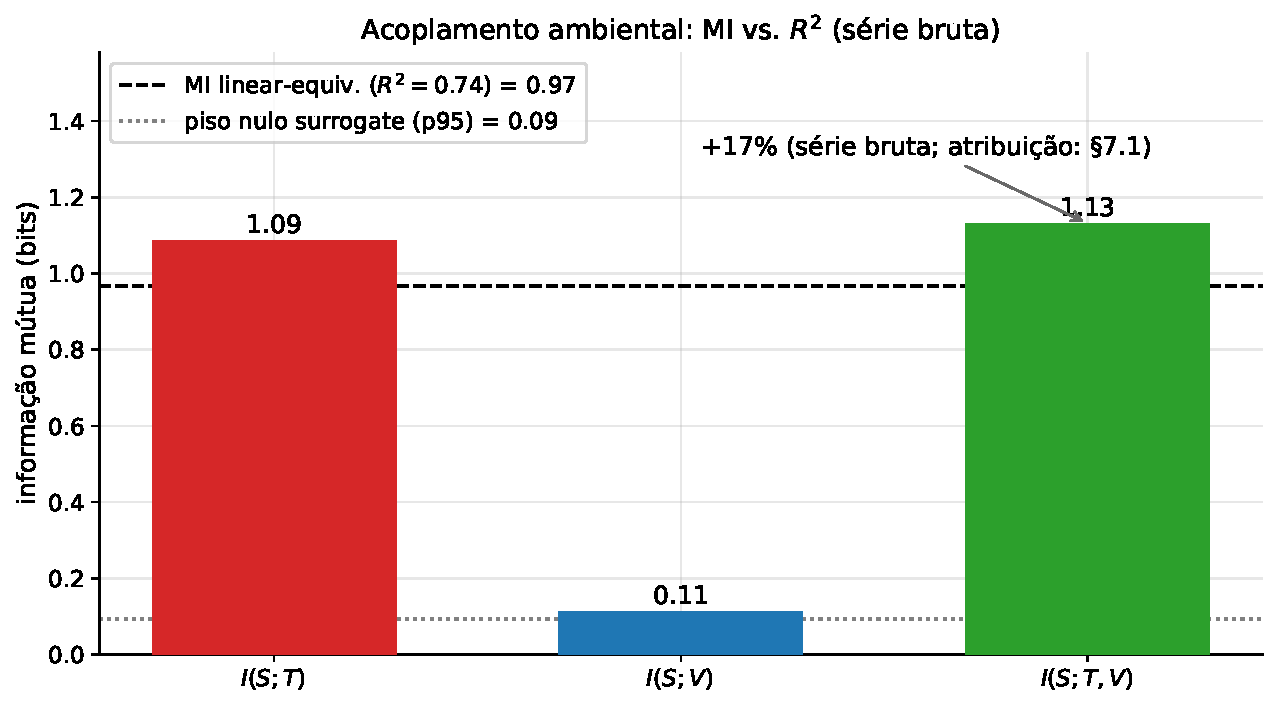
\includegraphics[width=\linewidth]{fig_mi_slide.pdf}
    \end{column}
  \end{columns}
\end{frame}

%------------------------------------------------------------------------------
\begin{frame}{O pilar da honestidade: $\neff$}
  \begin{itemize}
    \item \valPostSoakSamples{} amostras brutas é \alert{enganoso}:
          $\tauint = \valTauInt$~s ($\sim$5\,min de decorrelação).
    \item Tamanho efetivo de amostra $\;\neff = \alert{\valNeff}\;$ (não 768{,}884).
    \item Todo intervalo de confiança, o piso \emph{surrogate} e o ajuste
          Bayesiano usam $\neff$ --- nunca a contagem bruta.
  \end{itemize}
  \vfill
  \begin{alertblock}{Por que importa}
    A série 1\,Hz é fortemente autocorrelacionada. Reportar sobre $\neff$ com
    ICs por \emph{block-bootstrap} + um nulo \emph{surrogate} é a espinha
    dorsal metodológica.
  \end{alertblock}
\end{frame}

%------------------------------------------------------------------------------
\guidequestion{dá para remover?}% [TFinfo] fio condutor, slide 6
\begin{frame}{Correção PVT = \emph{denoise} + recuperação do envelhecimento}
  \begin{columns}[T]
    \begin{column}{0.5\textwidth}
      \begin{itemize}
        \item Acoplamento reversível $\valPreMIrev \rightarrow \valResidMI$~bits
              (\alert{$\valMIreductionPct\,\%$ removidos}); MDL seleciona o
              modelo \valCorrModel.
        \item \textbf{Chave:} remover PVT \emph{expõe} o envelhecimento ---
              $\operatorname{corr}(\slk,\tm)\;\valCorrStRaw \rightarrow \valCorrStCorr$.
      \end{itemize}
    \end{column}
    \begin{column}{0.5\textwidth}
      \centering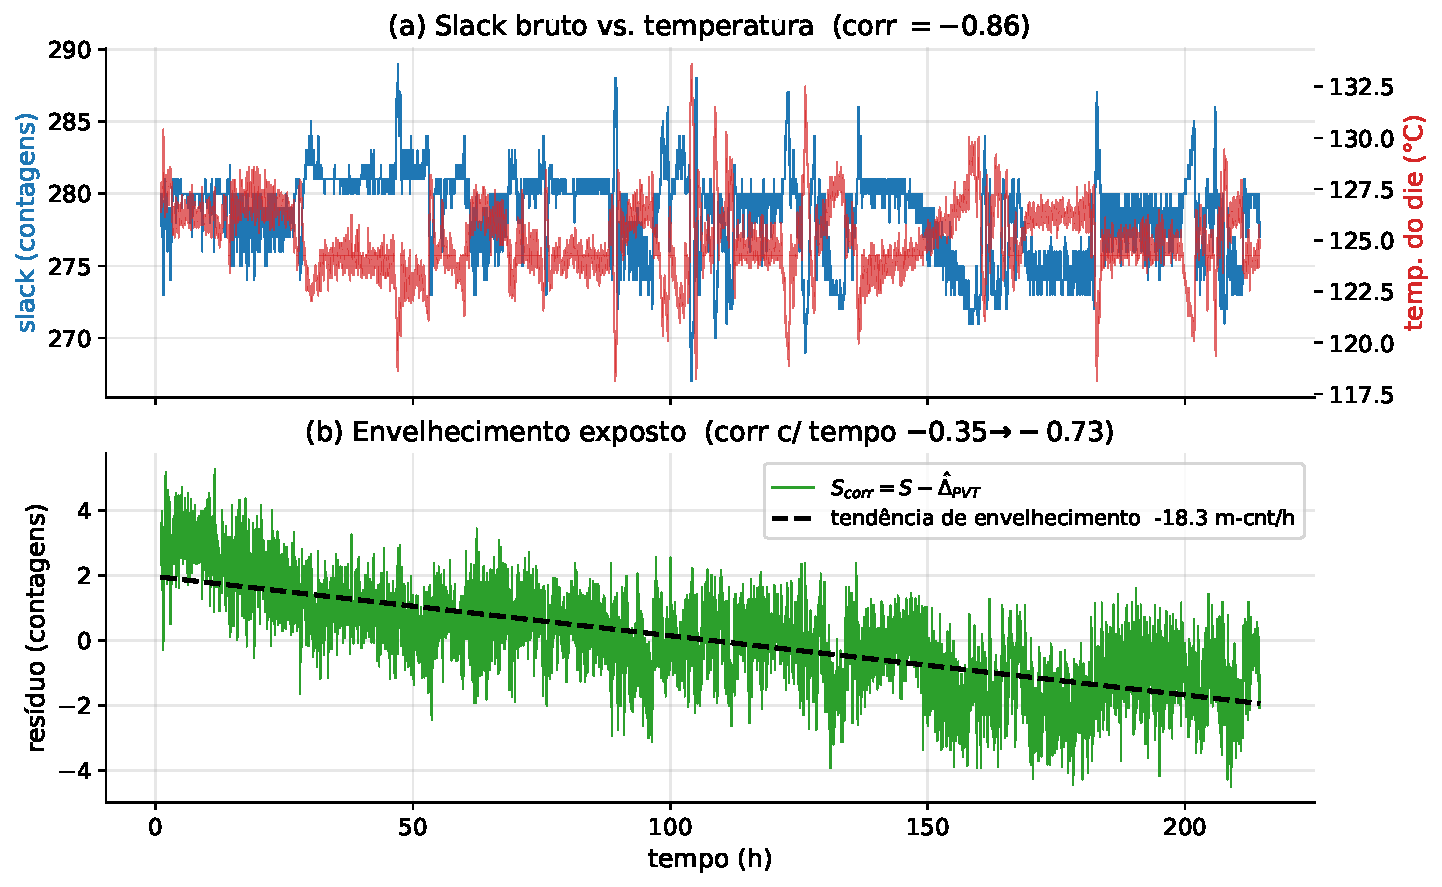
\includegraphics[width=\linewidth]{fig_correction_slide.pdf}
    \end{column}
  \end{columns}
\end{frame}

%------------------------------------------------------------------------------
\guidequestion{o que o sensor resolve?}% [TFinfo] fio condutor, slide 7
\begin{frame}{Resolução efetiva \& confiabilidade do alarme}
  \begin{columns}[T]
    \begin{column}{0.5\textwidth}
      \begin{itemize}
        \item $\mathrm{SNR} = \valSNR \Rightarrow C = \valCapacityBits$~bits
              $\Rightarrow \alert{\valCapacityStates}$ estados de envelhecimento distinguíveis.
        \item Alarme de envelhecimento (BSC): 1\,h $\approx$ lançamento de moeda;
              \alert{$\valBSCwindow$\,h $\rightarrow \Cbsc = \valBSCcap$~bits}.
        \item A transição coincide com o tempo mínimo de observação do CRLB.
      \end{itemize}
    \end{column}
    \begin{column}{0.5\textwidth}
      \centering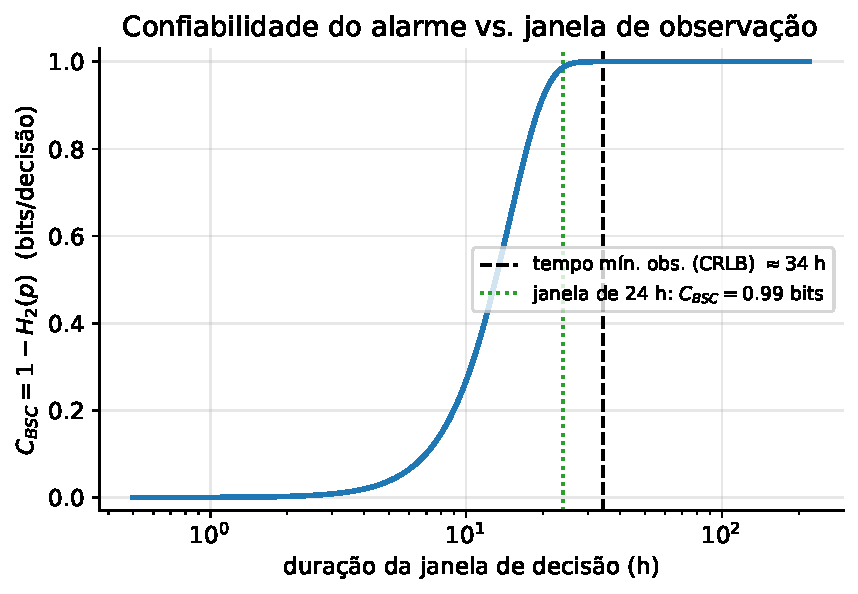
\includegraphics[width=\linewidth]{fig_capacity_rul.pdf}
    \end{column}
  \end{columns}
\end{frame}

%------------------------------------------------------------------------------
\guidequestion{quando o envelhecimento aparece?}% [TFinfo] fio condutor, slides 8–8b
\begin{frame}{Limite de detectabilidade de RUL}
  \begin{itemize}
    \item \textbf{Cram\'er--Rao:} taxa mín.\ detectável \alert{\valMinDetectRate~m-cnt/h};
          tempo mín.\ de observação \alert{\valMinObsTime~h}
          (execuções anteriores de $\sim$23\,h não separavam o envelhecimento).
    \item \textbf{Bayesiano:} inclinação $\valBayesSlope$~m-cnt/h,
          IC 95\% $[\valBayesSlopeLo,\valBayesSlopeHi]$;
          $P(\text{inclinação} < 0) \approx \valBayesPaging\,\%$.
    \item Frequentista $=$ Bayesiano $\Rightarrow$ robusto.
  \end{itemize}
  \vfill
  \begin{block}{Enquadramento}
    Um limite, limitado por ruído, sobre \emph{quando} o envelhecimento se
    torna observável --- \textbf{não} uma predição de vida útil.
  \end{block}
\end{frame}

%------------------------------------------------------------------------------
\begin{frame}{RUL como distribuição: Wiener/Kalman}
  \footnotesize
  \begin{itemize}
    \item Rota \emph{sequencial} sobre o mesmo $\scorr$: média em blocos até
          $\neff$ pontos, suavização Kalman/RTS de uma trajetória de
          envelhecimento \textbf{processo de Wiener}. MLE do ruído de taxa
          $\to\!0$ --- \alert{concorda com o MDL} (taxa suavizada
          $\valWienerRateEnd$ vs.\ CRLB/Bayesiano $\sim\!-18$~m-cnt/h).
    \item \textbf{Distribuição de RUL Gaussiana-inversa} em forma fechada:
          média/mediana $\valRULmeanNoise$/$\valRULmedianNoise$~h em
          $D{=}\sigma_{\text{noise}}$;
          $\valRULmeanSignal$/$\valRULmedianSignal$~h em $D{=}\sigma_{\text{signal}}$.
  \end{itemize}
  \centering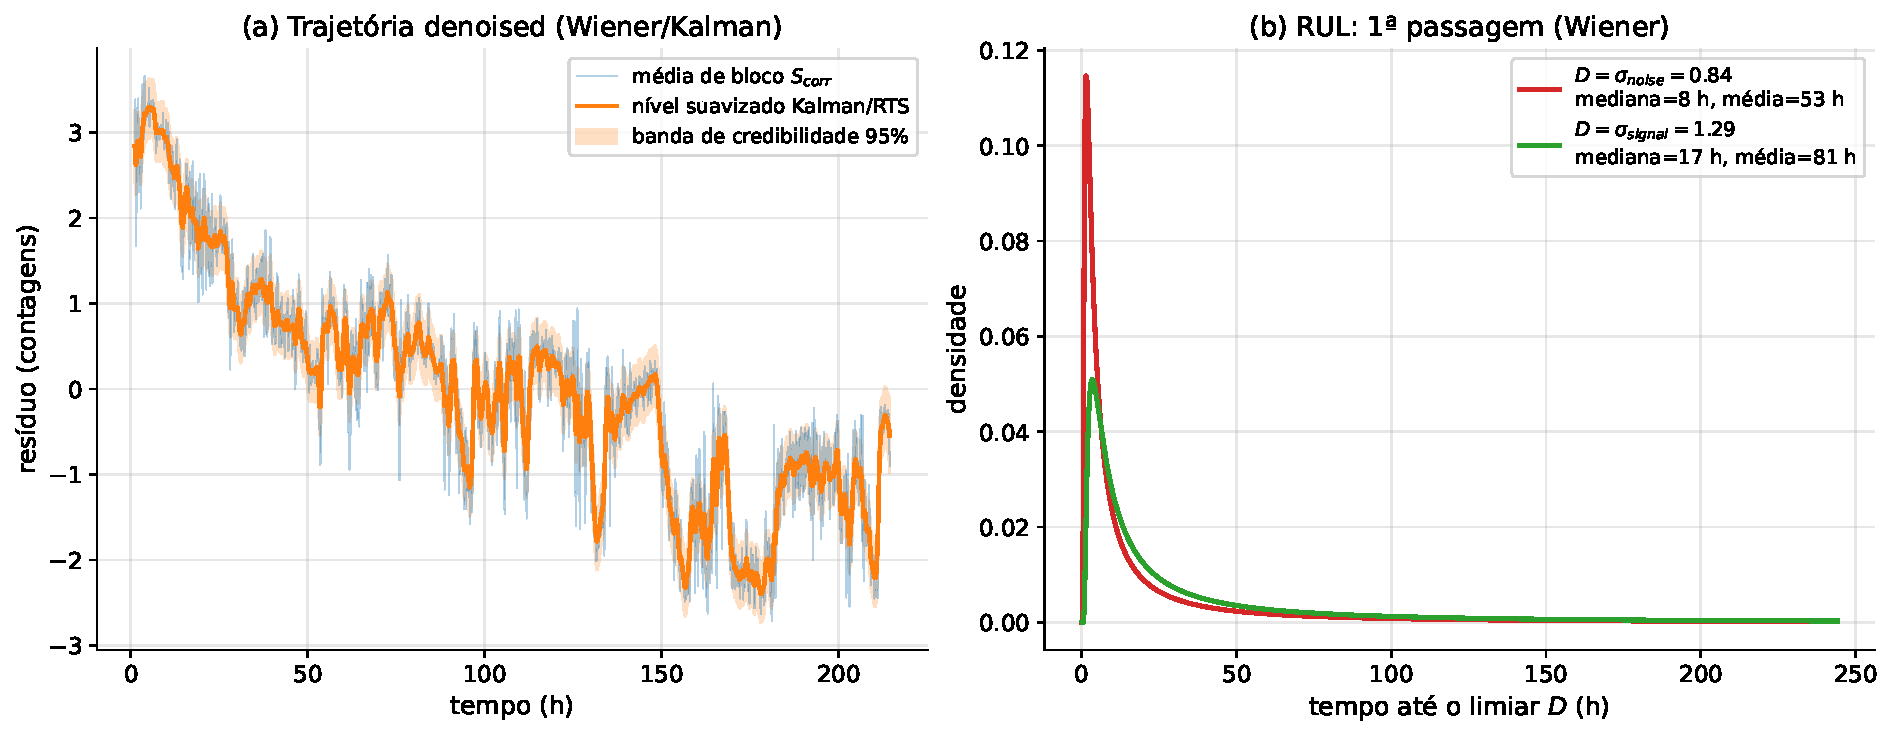
\includegraphics[width=0.76\linewidth]{fig_wiener_rul_slide.pdf}
\end{frame}

%------------------------------------------------------------------------------
\guidequestion{}% [TFinfo] limpa o fio condutor (conclusão)
\begin{frame}{Contribuições \& conclusão}
  \begin{itemize}
    \item Uma \textbf{métrica de contaminação em bits} (MI), sem hipótese de
          forma funcional e com unidade transferível entre sensores e bancadas.
    \item Uma \textbf{definição principiada de qualidade de \emph{burn-in}} $=$
          minimizar $\MI{\slk}{\Tdie,\Vcore}$, junto com um protocolo
          objetivo.
    \item Uma \textbf{especificação informacional do sensor}: $\valCapacityStates$
          estados resolvíveis, $\valBSCcap$~bits por decisão diária, e
          detectabilidade em $\valMinObsTime$~h --- explicando por que
          campanhas de $\sim$23\,h nunca foram suficientes.
  \end{itemize}
  \vfill
  \begin{alertblock}{Conclusão}
    $R^2$ diz que o ambiente explica $R^2=\valRsqLinear$ da variância. A
    teoria da informação diz que ele escreve \textbf{\valMIstv~bits} em
    cada leitura --- e, do acoplamento reversível
    ($\valPreMIrev\to\valResidMI$~bits), removemos
    \textbf{\valMIreductionPct\,\%}. Bits são transferíveis; frações de
    variância não são.
  \end{alertblock}
\end{frame}

\end{document}
